%!TEX root = ../../dissertation.tex
%%%%%%%%%%%%%%%%%%%%%%%%%%%%%%%%%%%%%%%%%%%%%%%%%%%%%%%%%%%%%%%%%%%%%%%%%%%%%%%%
\section{Measurements}
\label{c3:sec:measurements}

With these playback models at hand, this section demonstrates how to conduct actual evaluations of reliable streaming protocols with it.

As discussed, there are numerous incarnations of reliable streaming protocols in use. Almost all of them follow the same basic approach but with slight variations in execution and choice of playback strategies and corresponding parameters. But it is exactly these choices that can have a large impact on the streaming process and resulting quality. 

The problem lies in comparing these protocols to each other. Each of them is usually tied to a specific --- and most often proprietary closed source --- streaming player. Setting up all these players in one testbed is a huge effort and requires very specific software environments to be used on the client machines. Moreover, these players are built with user interaction and not automation and directly measuring the outcome in mind. This can still be achieved through extensive workarounds, but must be tailored to every player application. The presented approach avoids this hassle and provides a concise way to test any conceivable playback strategy in one single test setup.


%%
\subsection{Progressive Streaming Measurement Framework}

To enable quick evaluations for progressive streaming the framework follows a two phase approach, separating the active online recording phase from the passive playback emulation. Recording data is very time intensive and cannot be sped up when conducting investigation of a real world process, and not relying on simulated data. It still replicates the steps a user would perform to consume a media stream on a playback device. Through appropriate configuration different scenarios can be modeled, e.g. network conditions, behavior and specifics of the user device.
 
\begin{figure}[htb]
    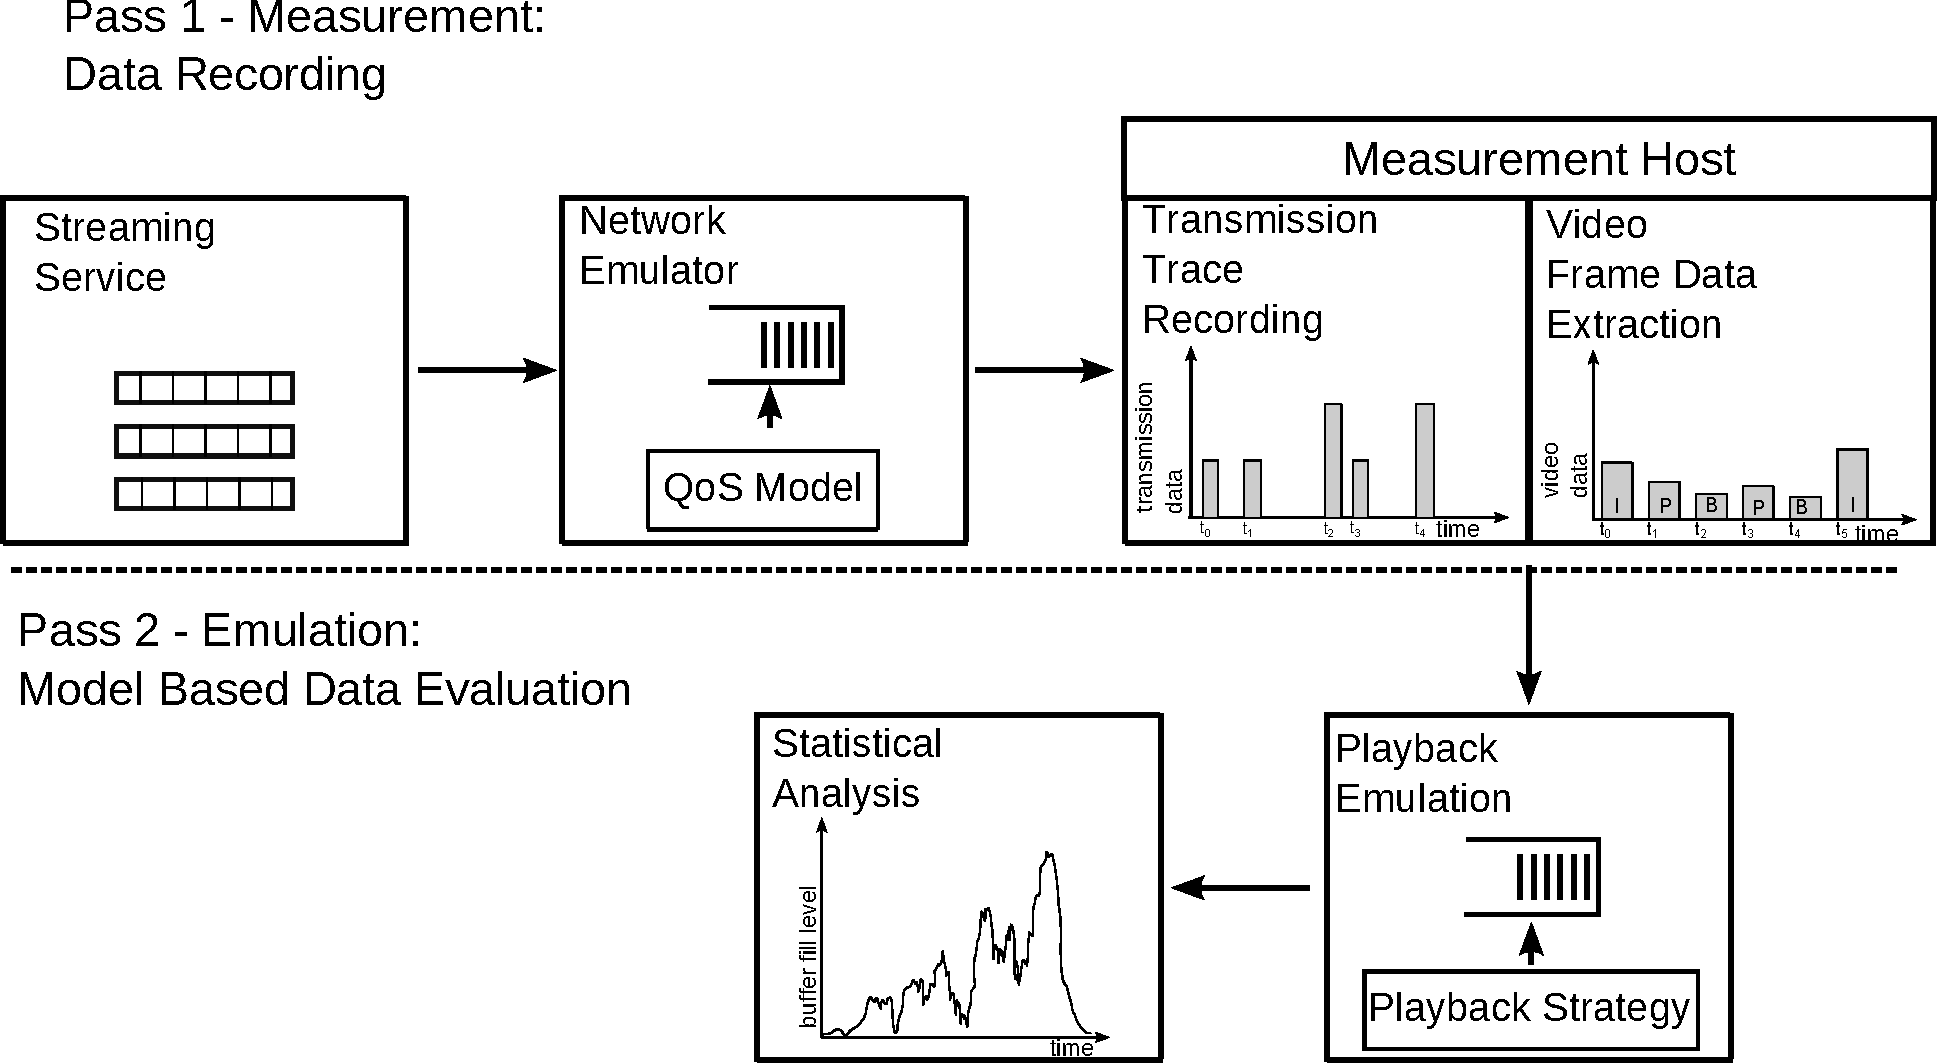
\includegraphics[width=\textwidth]{images/measurement-model.pdf}
    \caption{Measurement framework for progressive streaming playback strategies overview.}
    \label{c3:fig:framework}
\end{figure}

Figure \ref{c3:fig:framework} depicts the framework for a streaming evaluation testbed. In phase one the stream's transmission is conducted and recorded on a per-packet level. Stream data is transmitted to the client from a server which can be any actual streaming service on the Internet or a local server under the testbed's control, eliminating undesired side effects caused by the Internet connection. 

The traffic is directed through a network emulation node capable of altering the network \gls{QoS} parameters, i.e. latency, jitter, and packet loss. The parameters can be set according to stochastic models derived from actual network architectures. Instead of network emulation, any preexisting architecture can also be placed here to achieve more accurate results for the intended target. This is especially helpful for complex infrastructures hard to model or with no good and concise models available yet, for example mobile and mobile core networks with the influence of encapsulating traffic into bearers.

The measurement host downloads and records the video stream as a network trace. For progressive \gls{HTTP} streaming, a single request on the video file is issued and the \gls{TCP} connection maintained until the file has fully arrived.
This process is recorded as basis for the second phase. These traces should consist of the size and timestamp of every incoming packet. More detailed traces can be used to scrutinize other layers of the connection, e.g. the dynamics of TCP receive window size. Additionally the received file is decoded yielding a trace of all video frame sizes and playout timestamps.

In the second pass, these two traces are then used to feed the actual reliable streaming playback model described before. This conducted by a closed-loop emulation process calculating the current buffer fill level based on the collected transmission and video frame traces for every point in time. 

All of the progressive streaming --- i.e. non-adaptive --- strategies can be tested on the same trace set.
In simple \gls{HTTP} streaming, the transmission is not controlled by the streaming application and no rate control is conducted. Therefore, recording the packet trace and simulating playback are completely decoupled, as the latter cannot influence the former.  This enables fast and efficient comparison of non-feedback protocols subject to the same network conditions.

The emulator then generates playback stalling statistics, specifically their number and duration, to compare the effect of the different strategies on the same trace. With these results, parameter settings for playback strategies can also be iteratively tested and improved leading to an empirical calibration of playback strategies instead of relying on best practices.

One of the drawbacks of this model-based emulation approach is of course the reliance on suitable models and playback strategies for the stream protocols under scrutiny. Obtaining these from proprietary streaming clients, can be a difficult reverse-engineering process.


%%
\subsection{Adaptive Streaming Measurement Framework}

Up to this point, the measurement framework is only suitable for progressive streaming omitting any adaptive strategy. This second framework modifies this and additionally allows for the testing of adaptive playback strategies. However, to achieve this, the advantageous two phase setup cannot be employed anymore.

\begin{figure}[htb]
    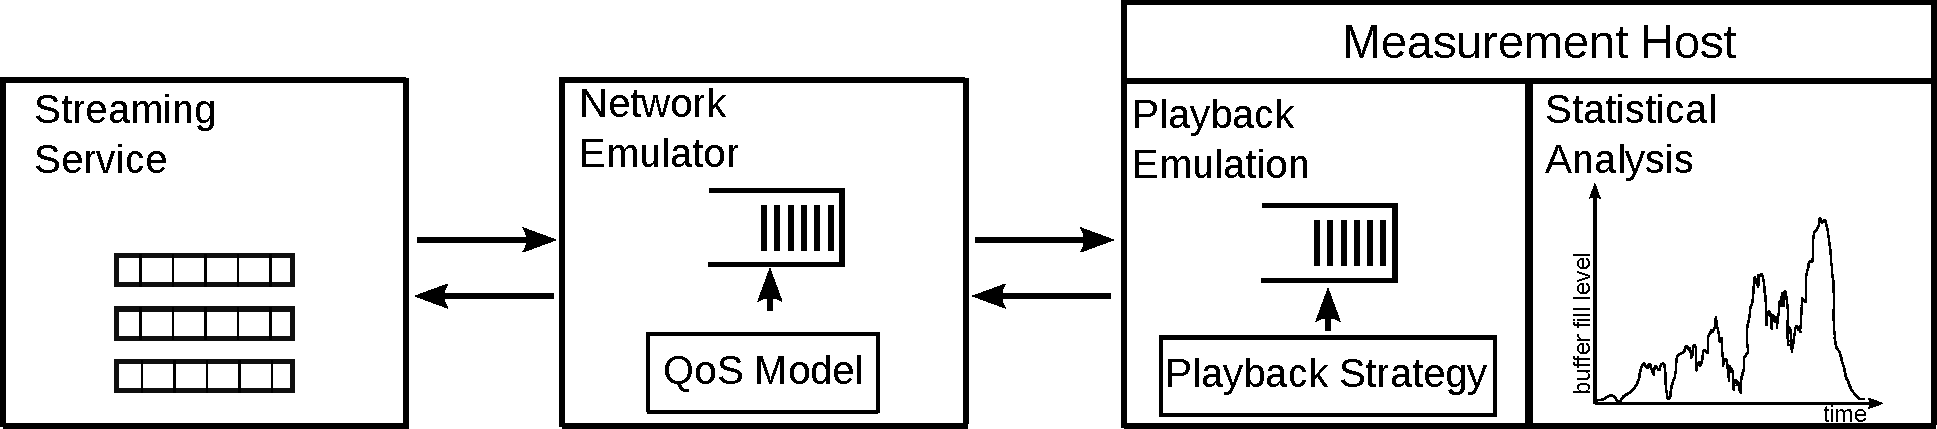
\includegraphics[width=\textwidth]{images/feedback-measurement-model.pdf}
    \caption{Measurement framework for adaptive streaming playback strategies overview.}
    \label{c3:fig:framework-feedback}
\end{figure}

Figure~\ref{c3:fig:framework-feedback} shows the adapted framework. The playback emulation process is now directly fed with the stream transmission without recording it first. The emulation is now an online process and has to be conducted in realtime. This enables the emulator to react on the current streaming state and request an alteration from the server. The adaptation spectrum ranges from the timing of stream segment retrieval to the chosen quality level of future segments. 

While allow for a wider range of playback strategies, this approach is also inherently slower as it does not allow a speed-up beyond realtime, limiting its usability somewhat. Therefore, a transition to a full simulative approach is suggested. This is path is further explored and discussed in Section~\ref{c6:sec:mobilestreamingtestbed}.

\todo{check simulation approach ref or further explain simulation}


%%
\subsection{Technical Implementation}

To conduct measurements, the described two phase progressive streaming measurement framework was implemented in a testbed. This testbed consists of three interconnected physical nodes running Linux. 

The optional streaming server houses an Apache httpd\footnote{\url{https://httpd.apache.org/}} Web server, hosting the files that are to be streamed. Alternatively, Internet streaming service traffic can also be directly routed through the network emulation node.

The network emulation node uses the existing \gls{QoS} capabilities of the Linux kernel, dubbed NetEm \cite{hemminger2005network}, to add latency and packet loss to the transmission as well as to act as a bandwidth bottleneck. The additional delay is set deterministically, the loss follows a uniform distribution without any correlation in the transmission.

To both retrieve the streaming file and record the transmission process at the client, curl\footnote{\url{http://curl.haxx.se/}} is used. If so desired, tcpdump\footnote{\url{http://www.tcpdump.org/}} can also be facilitated to achieve a higher recording precision. The video file is then parsed for its frames and sizes using mplayer\footnote{\url{http://www.mplayerhq.hu/}} with libav\footnote{\url{https://libav.org/}}. The traces are then put into the actual playback emulation, implemented by custom Python-based code and statistically evaluated with Python as well as R.



%%
\subsection{Measurement Series and Evaluations with the Framework}

This implementation has been used to conduct a comparative study of two theoretical and two real world playback strategies. They are tested for their susceptibility to worsening network \gls{QoS}, latency and loss in this case. The evaluated strategies are the described YouTube and Firefox strategies as well as the null strategy and the predictive strategy with perfect knowledge and just the initial stalling period.

The video used in the experiment was streamed from the YouTube web site providing a realistic foundation for the experiments. This also enables a server side pacing mechanism adjusted to the video bitrate for free.
Details on the video used in the experiment are available in Table~\ref{c3:tbl:videoparams}. Two measurement series are performed with this video, both only differ in the network emulator setting. The first series increasingly adds packet loss to the stream, with the second series altering the packet delay. In both scenarios, the link bandwidth was limited to a typical dialup value of \SI{16}{\mega\bit\per\second} in the downlink direction and \SI{1}{\mega\bit\per\second} up.

It can be stated, that all playback strategies will generally work very similar under good network conditions as long as the \gls{TCP} goodput, i.e. the rate the payload is transported by \gls{TCP}, is higher than the video bitrate. With sufficient goodput video streams will start with almost no delay or intermediate buffering. 
If, however, the achievable \gls{TCP} goodput is close to the average video bitrate, the buffer can be quickly drained by short deviations from the average transmission and video bit rates. The \gls{TCP} goodput can be limited by high latency and loss. Many \gls{TCP} congestion control algorithms depend on the round trip time. If the \gls{RTT} is high, the congestion window will increase much slower. High latency triggers \gls{TCP} timeouts and retransmissions, and in turn decrease the congestion window reducing the goodput. Packet loss affects \gls{TCP} goodput even more. A lost packet results in duplicate acknowledgments followed by retransmissions and a decrease of the congestion window. The problem is worsened if the acknowledgments are also lost. The connection could stalls on missing old segments without which the playback cannot proceed. In addition to the reduction of goodput this results in a delay burst and high jitter for the streaming application.


\begin{table}[htbp]
    \centering
    \caption{Test Video Parameters}
    \label{c3:tbl:videoparams}
    \begin{tabu}{X[l]X[r]}
        \toprule
        \textbf{Parameter} & \textbf{Value} \\
        \midrule
        Video Duration  & \SI{92.536}{\second}\\
        Size & \SI{9.61}{\mebi\byte} \\
        Frame rate & \SI{23.976}{\per\second} \\
        Average Video Bitrate & \SI{871}{\kilo\bit\per\second} \\
        Codecs & AVC+AAC \\
        \bottomrule
    \end{tabu}
\end{table}


%% latency
In the latency measurement series, the emulator delays forwarding the packets for a constant amount of time. The latency was increased in \SI{100}{\milli\second} steps, up to a total of \SI{5000}{\milli\second}. The added latency is split up evenly between the uplink and the downlink.

\begin{figure}[htb]
    \centering
    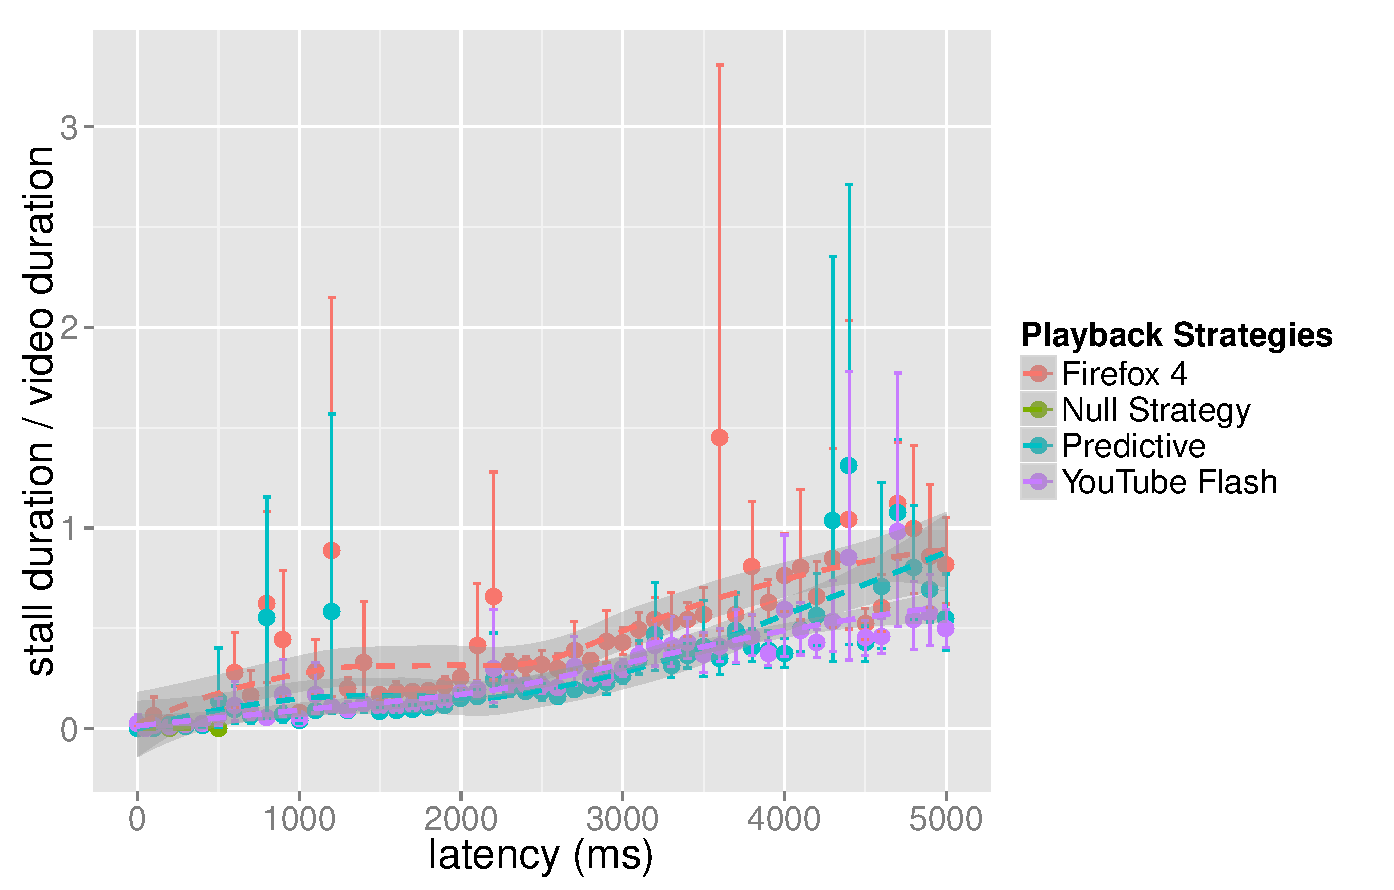
\includegraphics[width=0.9\textwidth]{images/R-playbackemulation-stallduration-latency.pdf}
    \caption{Stalling duration in relation to transmission latency with local polynomial least-squares fit.}
    \label{c3:fig:eval-latency-stallingtime}
\end{figure}


Figure~\ref{c3:fig:eval-latency-stallingtime} depicts the relation between the added latency and the stalling duration of the playback strategies. The stalling time increases as expected with the additional latency, but Firefox's strategy seems to have slight edge during high latency. Overall, the stalling duration quickly reaches a length comparable to the actual video duration and even surpassing that. Someone watching a stream under this condition might find this not acceptable any longer.
% Both the predictive and the null strategy provide the best possible result in terms of pure stalling time. This was already theoretically explored during the strategy's introduction. <-- not true, why?


\begin{figure}[htb]
    \centering
    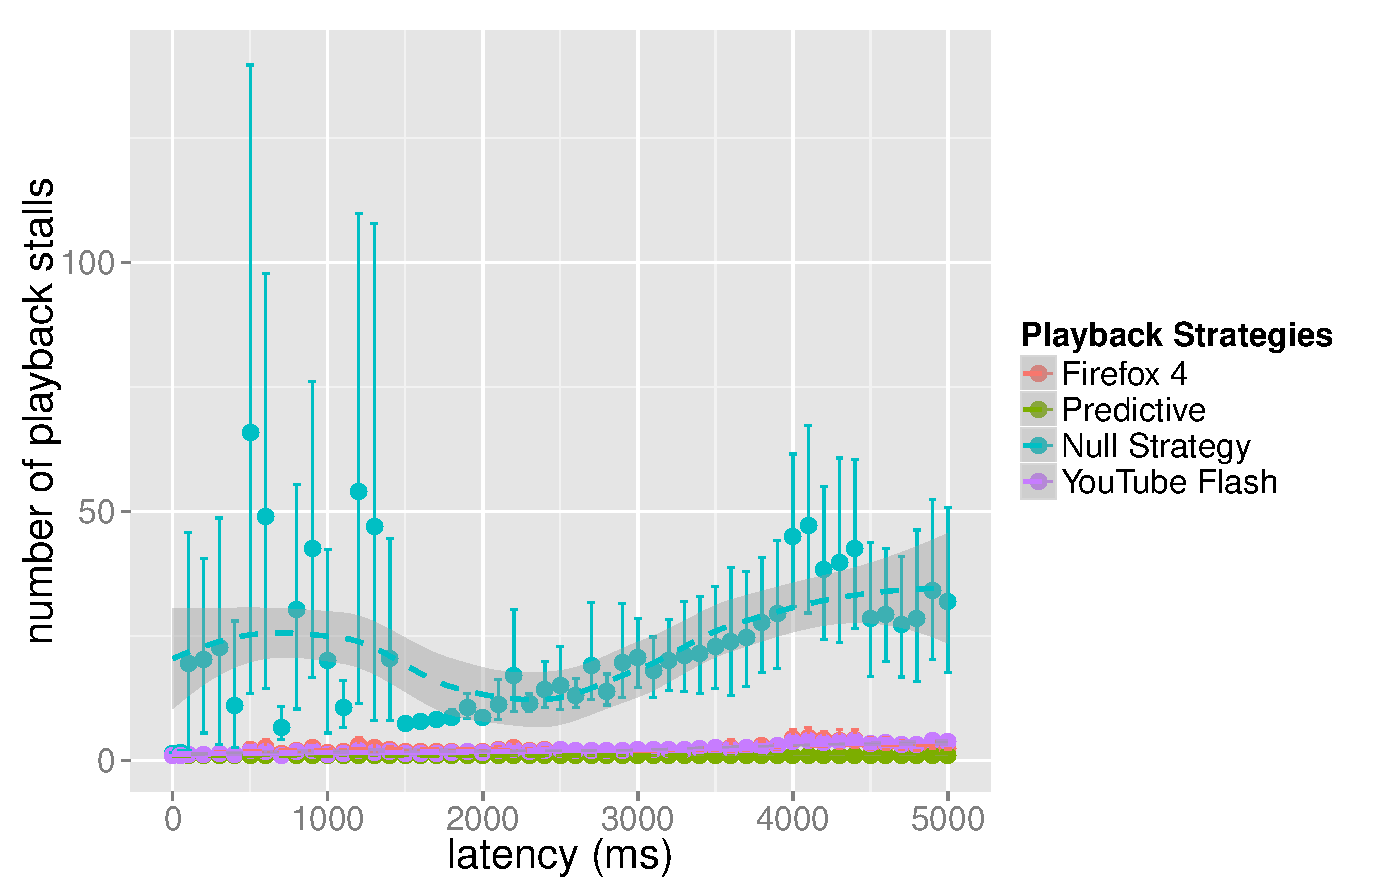
\includegraphics[width=0.9\textwidth]{images/R-playbackemulation-stallnumber-latency.pdf}
    \caption{Number of stalls in relation to transmission latency with local polynomial least-squares fit.}
    \label{c3:fig:eval-latency-numstalls}
\end{figure}

Figure \ref{c3:fig:eval-latency-numstalls} additionally shows number of stalling events occurring during the playback with the null strategy at the high end and the predictive strategy just showing the expected single stall before playback start. %But both YouTube and Firefox are not much worse compared to the predictive strategy, running in just a few buffering events of increasing duration with rising latency. 
%YouTube stalling time is usually lower than with Firefox, at the cost of slightly more buffering events, which could be attributed to its optimistic threshold choice, which still seems to work at the tested latency levels.

Overall, it can be said, that in this specific latency scenario the real world playback strategies seem to honor the fact that more video interruption lead to a worse experience than fewer but longer ones.  Through mobility and handovers, mobile devices experience short bursts of latency of several seconds fairly common. According to the measurement series, the resulting stalling behavior could still very well be bearable for streaming users.

In the loss measurement series, uncorrelated and uniformly distributed loss was added in both the uplink and the downlink direction. The loss was incrementally increased in \SI{2}{\percent} steps up to a total additional loss of \SI{12.5}{\percent}. About \SI{4}{\percent} of the individual experiments did not finish correctly, and the video was not completely transmitted. This was caused by the \gls{TCP} stack, which at some point terminated the connection after to many packets were lost back to back, and curl giving up after several retries. This unpredictability and failure rate also leads to the high variability seen in the results of the loss measurement series. Nonetheless, a certain trend can still be derived from the results.


\begin{figure}[htb]
    \centering
    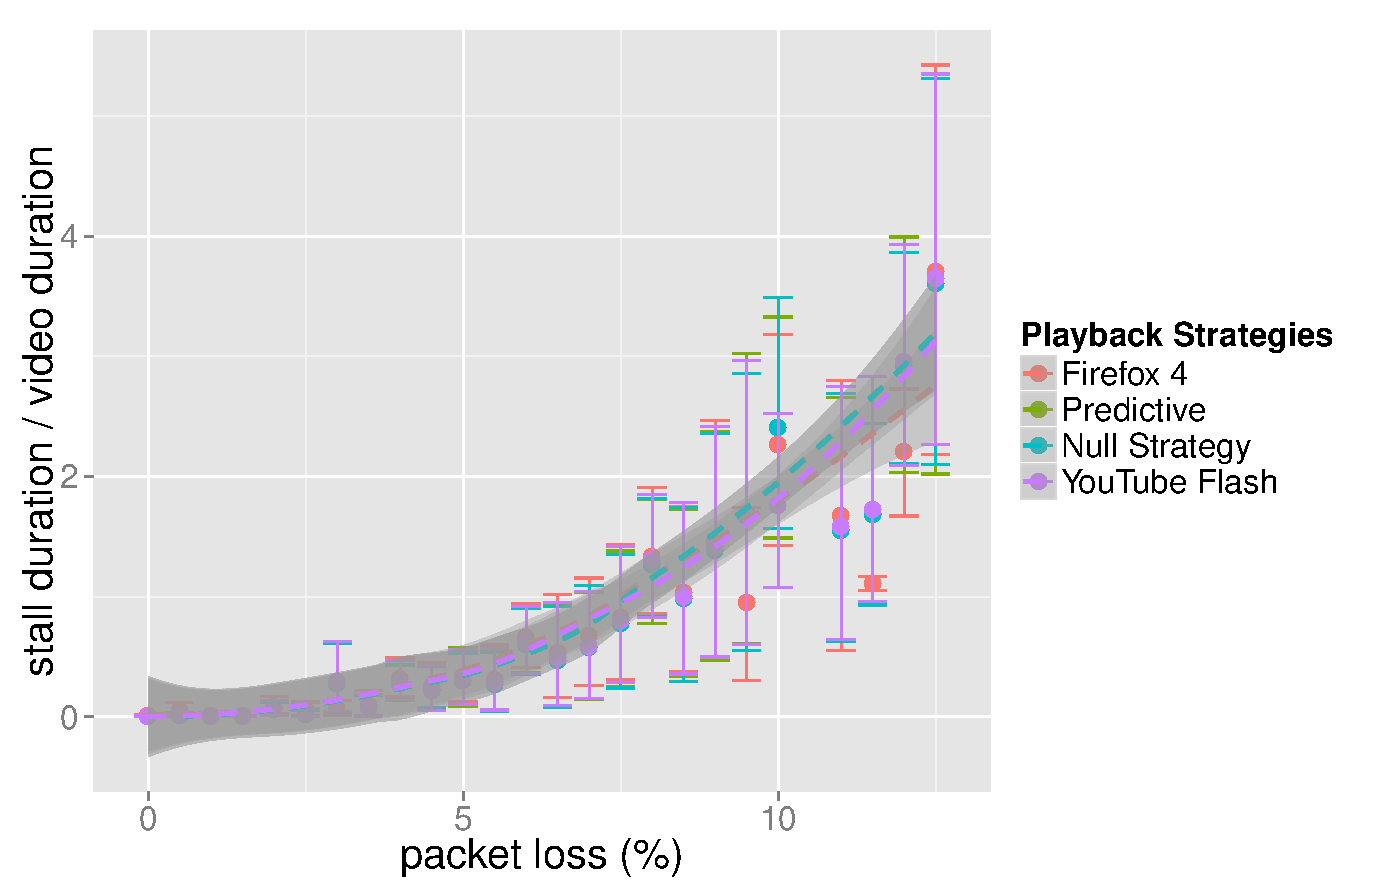
\includegraphics[width=0.9\textwidth]{images/R-playbackemulation-stallduration-loss.pdf}
    \caption{Stalling duration in relation to packet loss with local polynomial least-squares fit.}
    \label{c3:fig:eval-loss-stallingtime}
\end{figure}


Figure~\ref{c3:fig:eval-loss-stallingtime} shows the resulting relative stalling duration in the packet loss measurement series. Loss of up to\SI{4}{\percent} seems to have no discernible impact on the streaming process. Anything beyond this point sees a large increase in the stalling duration. With a relative stalling duration of almost four times the actual video length at \SI{12}{\percent} packet loss any streaming attempt is practically rendered unusable. This behavior could hint to the transport protocol's reliable transport feature, catching any occurring loss. However, the detection and retransmission takes time and leads to a bursty increase in latency offering a possible reason of the increased stalling time.


\begin{figure}[htb]
    \centering
    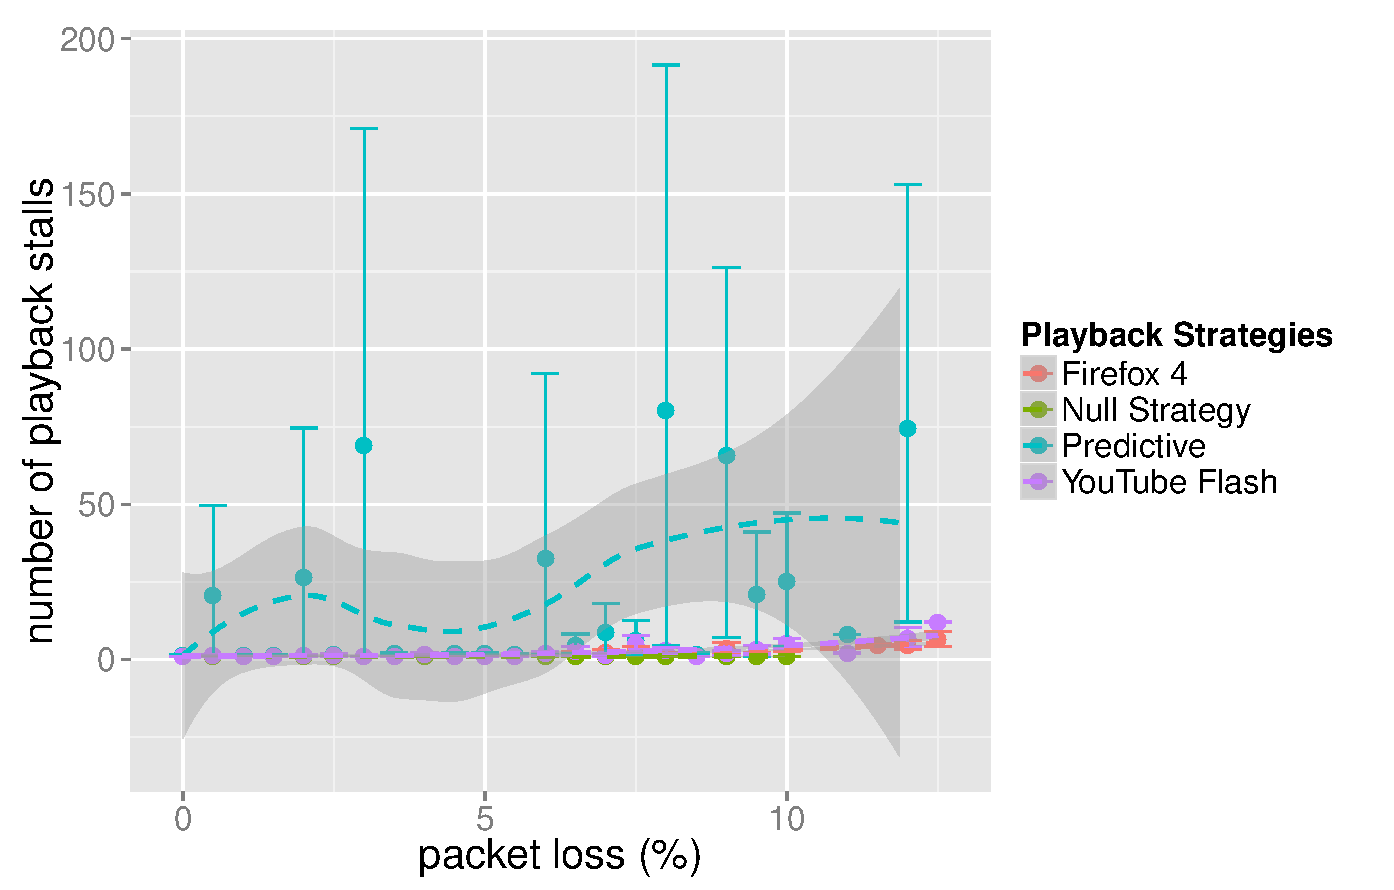
\includegraphics[width=0.9\textwidth]{images/R-playbackemulation-stallnumber-loss.pdf}
    \caption{Number of playback stalls in relation to packet loss with local polynomial least-squares fit.}
    \label{c3:fig:eval-loss-numstalls}
\end{figure}


Figure~\ref{c3:fig:eval-loss-numstalls} shows the extremity of the null strategy in terms of the number of experienced stalls compared to other strategies reaching a number two orders of magnitude larger than any other model. 


As a result, when planning a network for streaming applications, the maximum loss should be kept below the \SI{4}{\percent} mark to achieve reasonable streaming quality. 

\todo{expand loss section a bit more}


%% original python plots
% \begin{figure}[htb]
%     \centering
%     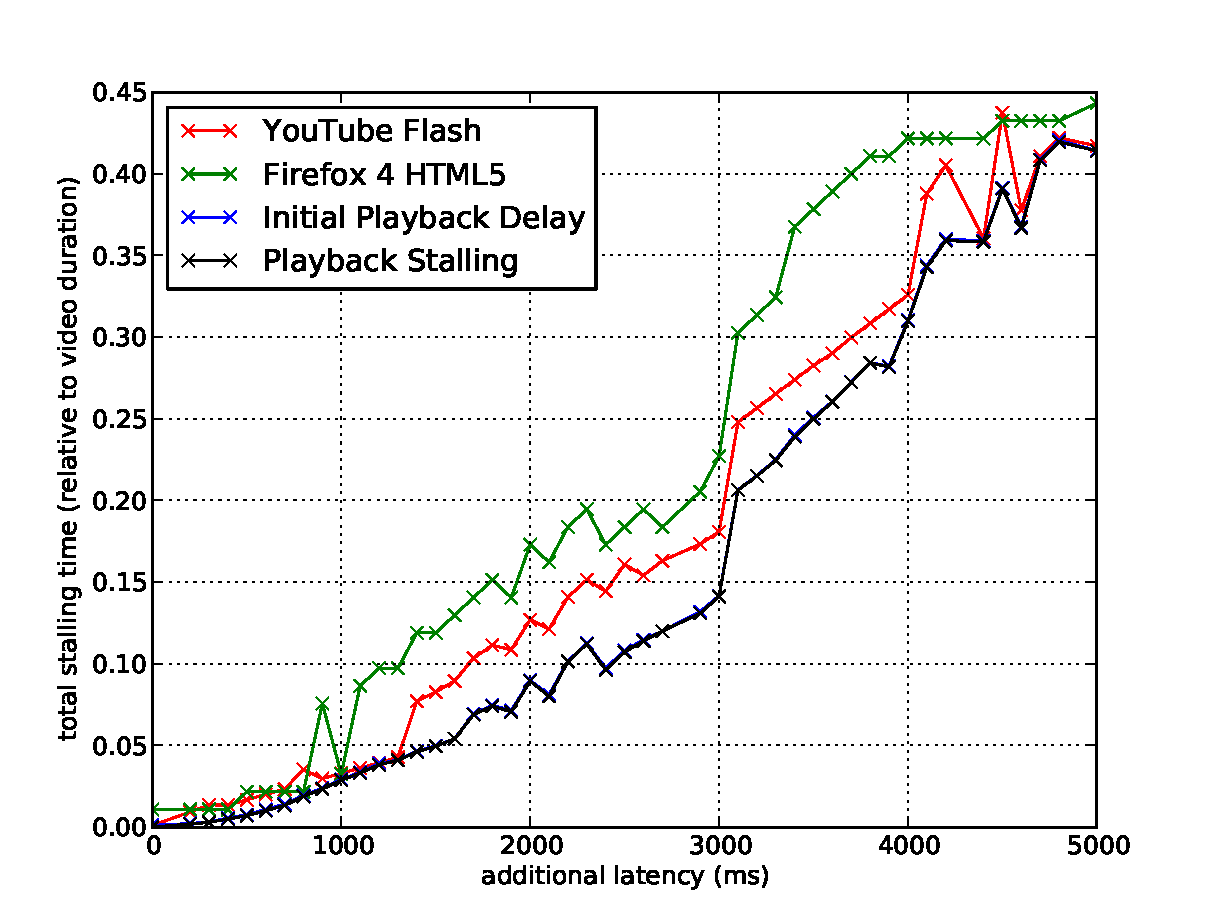
\includegraphics[width=\textwidth]{images/eval-latency-stallingtime.pdf}
%     \caption{Stalling duration in relation to transmission latency.}
%     \label{c3:fig:eval-latency-stallingtime}
% \end{figure}

% \begin{figure}[htb]
%     \centering
%     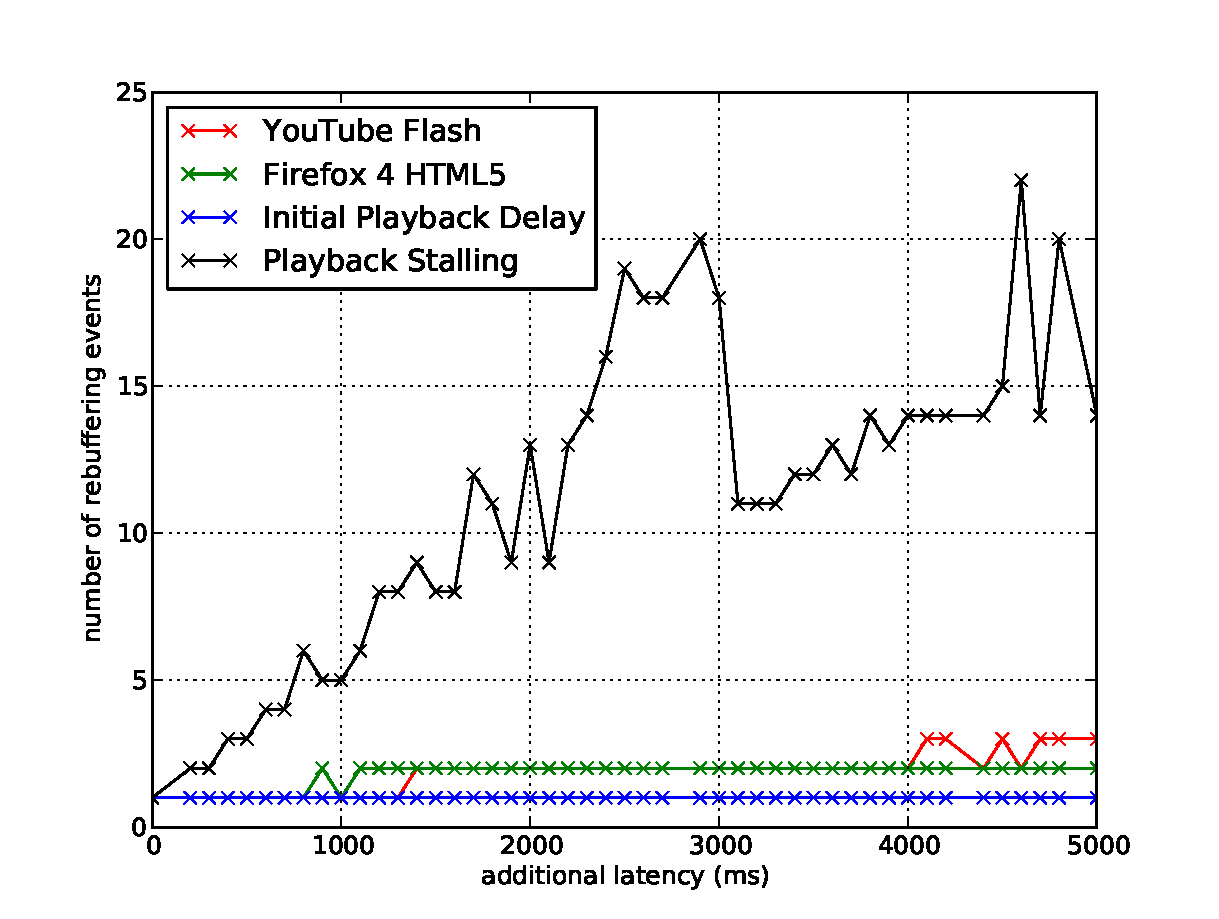
\includegraphics[width=\textwidth]{images/eval-latency-frequency.pdf}
%     \caption{Number of stalls in relation to transmission latency.}
%     \label{c3:fig:eval-latency-numstalls}
% \end{figure}

% \begin{figure}[htb]
%     \centering
%     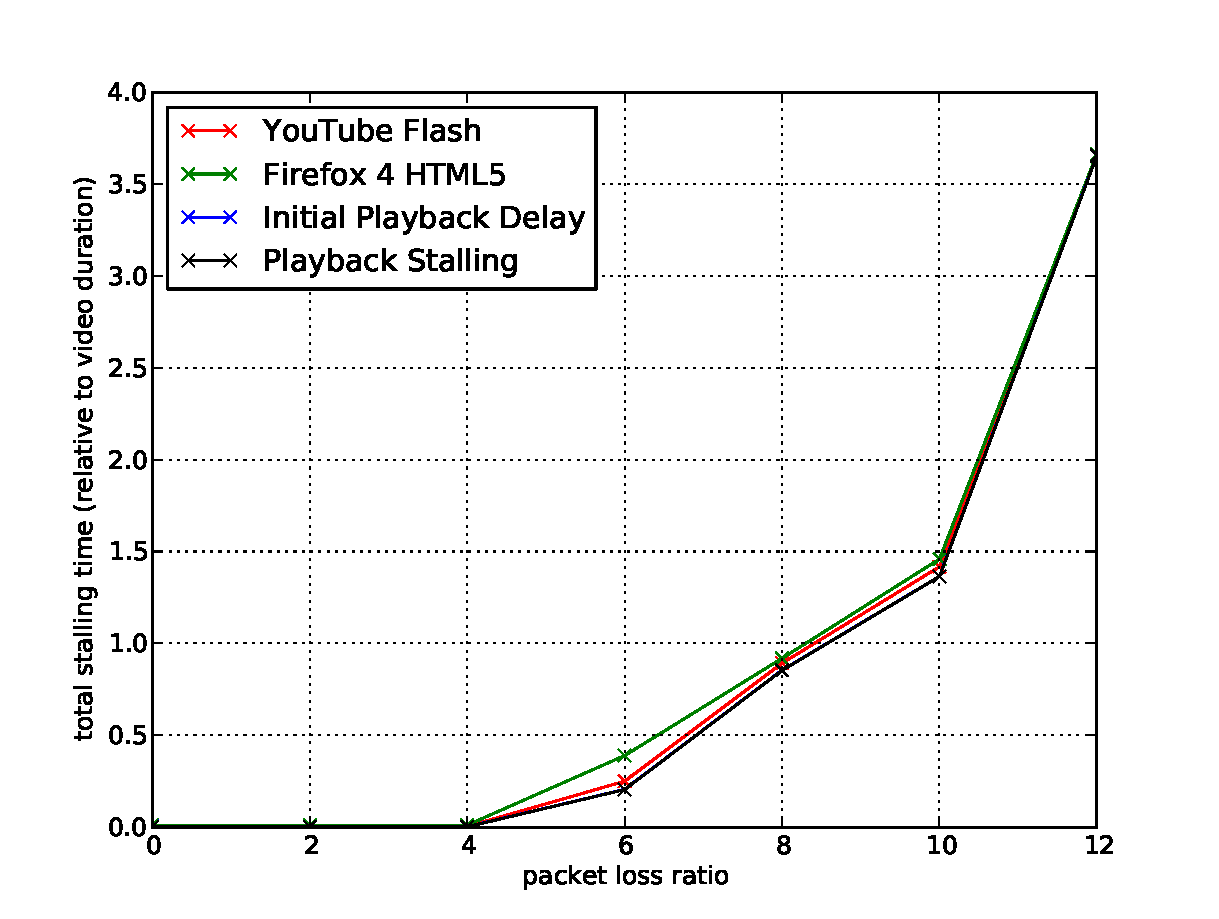
\includegraphics[width=\textwidth]{images/eval-loss4mb-stallingtime.pdf}
%     \caption{Stalling duration in relation to packet loss.}
%     \label{c3:fig:eval-loss-stallingtime}
% \end{figure}

% \begin{figure}[htb]
%     \centering
%     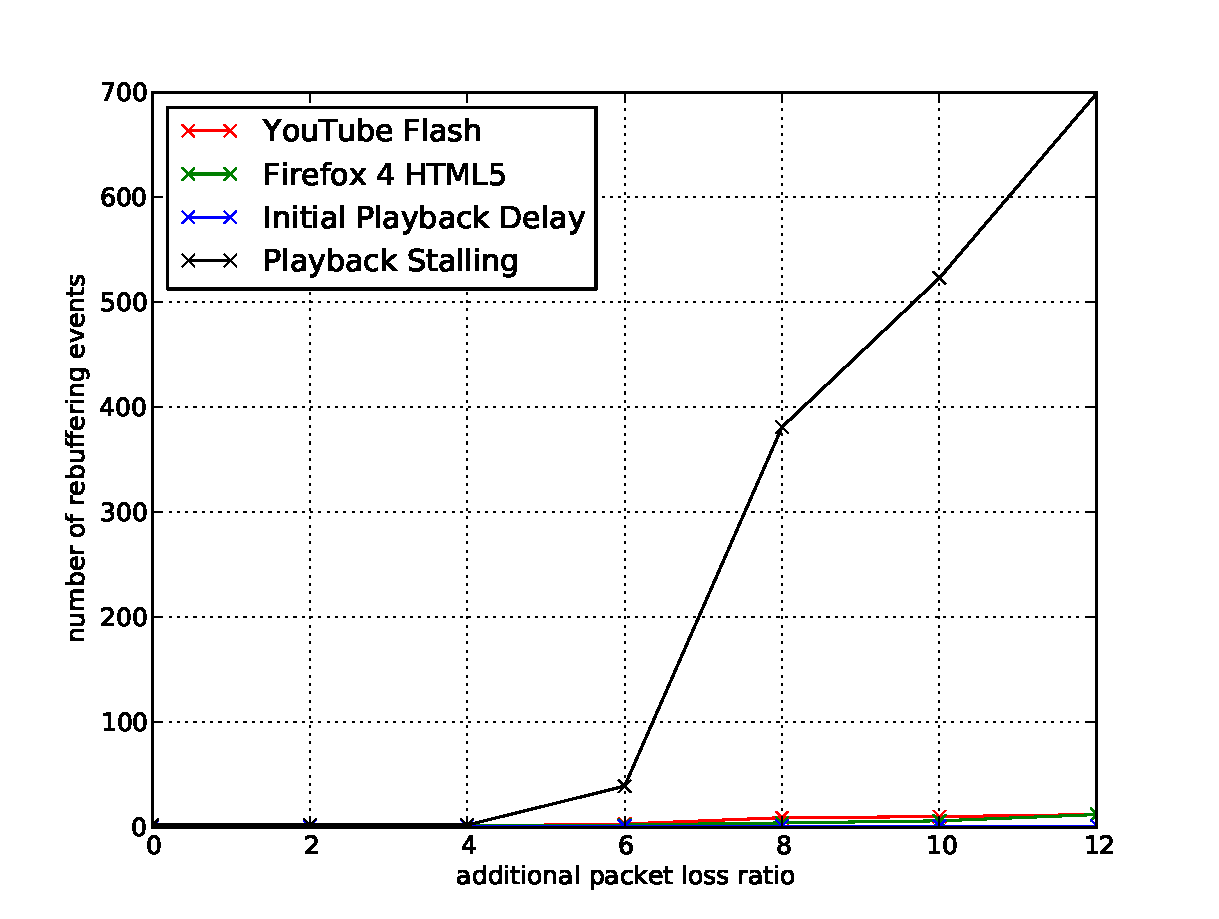
\includegraphics[width=\textwidth]{images/eval-loss4mb-frequency.pdf}
%     \caption{Number of playback stalls in relation to packet loss}
%     \label{c3:fig:eval-loss-numstalls}
% \end{figure}


% \begin{figure}[htbp]
%     \centering
%     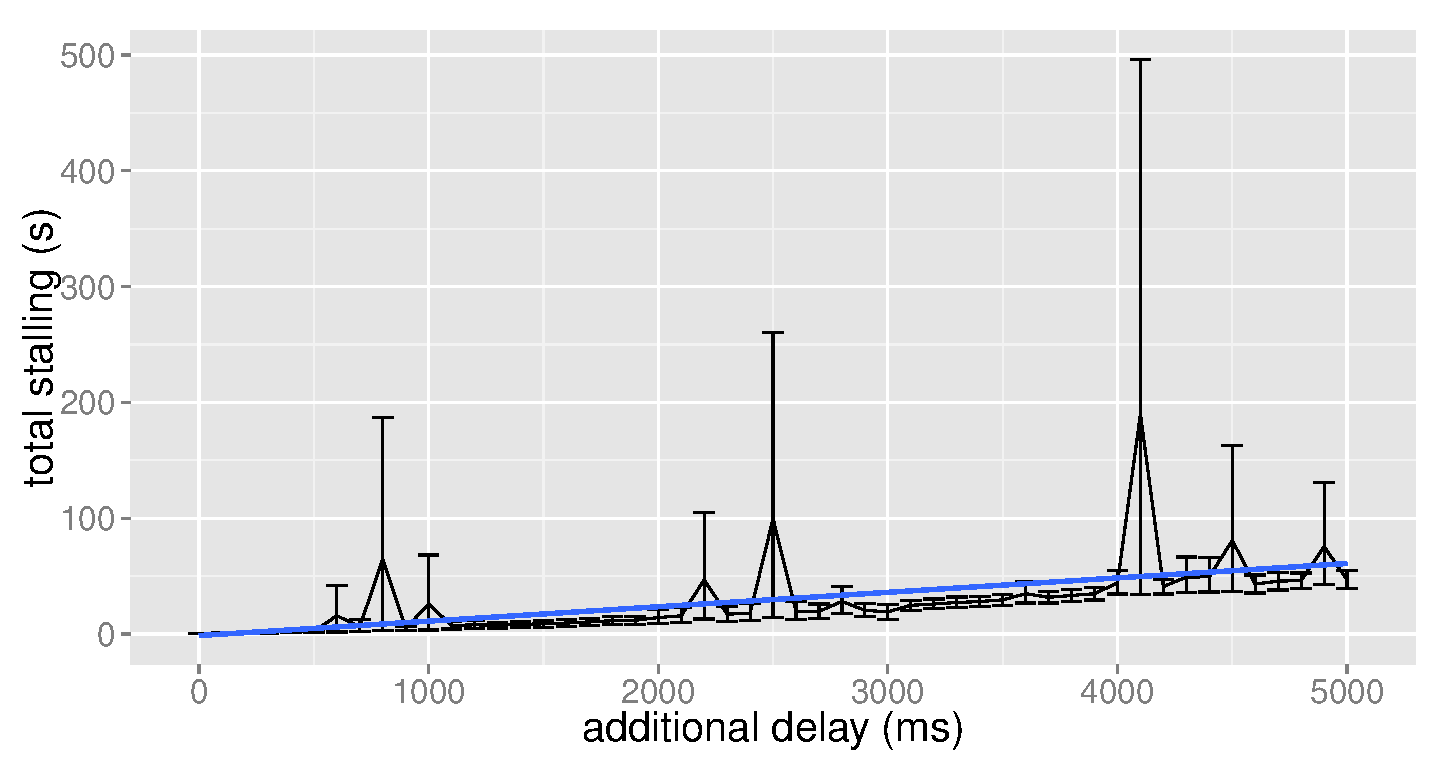
\includegraphics[width=\textwidth]{images/R-delayseries.pdf}
%     \caption{Total buffering time and linear smooth for degraded network parameter scenarios. Latency Graph.}
%     \label{c3:fig:delayseries}
% \end{figure}

% \begin{figure}[htbp]
%     \centering
%     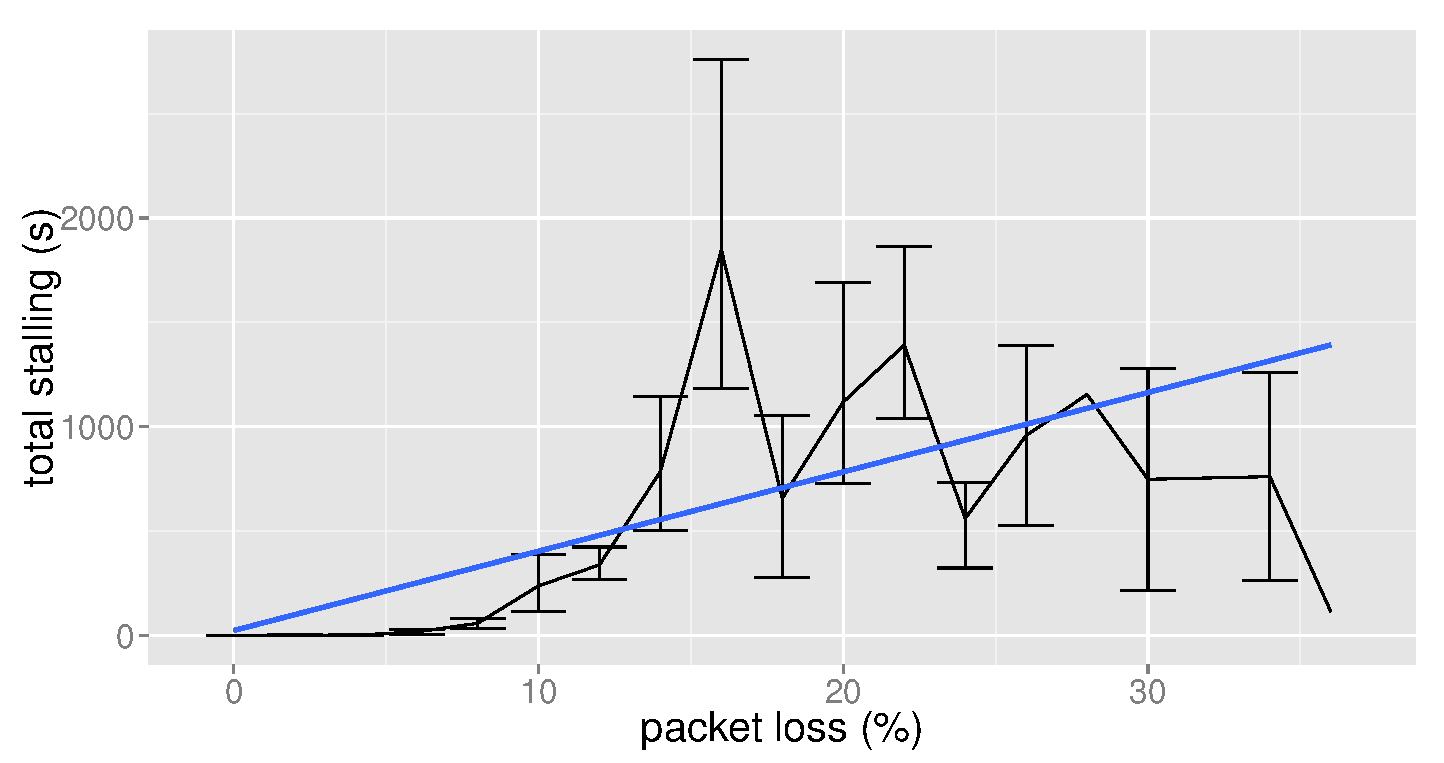
\includegraphics[width=\textwidth]{images/R-lossseries.pdf}
%     \caption{Total buffering time and linear model for degraded network parameter scenarios. Loss Graph.}
%     \label{c3:fig:lossseries}
% \end{figure}